\documentclass[]{article}
\usepackage{geometry}   % my added package "geometry"
\geometry{letterpaper,tmargin=1in,bmargin=1in,lmargin=2.2cm,rmargin=2.2cm}
\usepackage[colorlinks,bookmarksopen,bookmarksnumbered,
citecolor=green,urlcolor=red]{hyperref}
\hypersetup{pdfauthor={Name}}
%%%%%%%%%%%%%%%%%%%%%%%%%%%%%%%%%%%%%%%%%%%%%%%%%%%%%%%%%%%%%%%%%%%%%%%%%
%\usepackage{graphicx}
\usepackage{graphics}
\usepackage{epsfig}
\usepackage{epstopdf}
\usepackage{amsfonts}
\usepackage{amssymb}
\usepackage{booktabs}
\usepackage{color,soul}
\usepackage{subfig}
%%%%%%%%%%%%%%%%%%%%%%%%%%%%%%%%%%%%%%%%%%%%%%%%%%%%%%%%%%%%%%%%%
\usepackage{amsmath}
\usepackage{cleveref}
%\usepackage[fleqn]{amsmath}
\usepackage{lineno}
\usepackage{tikz}
\usepackage{standalone}
\usetikzlibrary{calc,patterns,arrows.meta,shapes.arrows,intersections,positioning}
\usetikzlibrary{decorations.pathmorphing,backgrounds,fit,petri}
\usepackage[percent]{overpic}
%%%%%%%%%%%%%%%%%%%%%%%%%%%%%%%%%%%%%%%%%%%%%%%%%%%%%%%%%%%%%%%%%
\usepackage{xcolor}
\usepackage{listings}
\lstset { %
	language=C++,
	backgroundcolor=\color{blue!5}, % set backgroundcolor
	basicstyle=\footnotesize\color{black},% basic font settingbasicstyle=\ttfamily\color{black}
	keywordstyle=\color{red},
	commentstyle=\color{violet},
	stringstyle=\color{blue},
	xleftmargin=2em,
	frame=single,
	framexleftmargin=2em,
	numbers=left,
	numberstyle=\tiny,
	numbersep=8pt,
}
%%%%%%%%%%%%%%%%%%%%%%%%%%%%%%%%%%%%%%%%%%%%%%%%%%%%%%%%%%%%%%%%%
\renewcommand\thesubsection{\thesection\Alph{subsection}}
%%%%%%%%%%%%%%%%%%%%%%%%%%%%%%%%%%%%%%%%%%%%%%%%%%%%%%%%%%%%%%%%%
\renewcommand\lstlistingname{Header}
\renewcommand\lstlistlistingname{Header}
%%%%%%%%%%%%%%%%%%%%%%%%%%%%%%%%%%%%%%%%%%%%%%%%%%%%%%%%%%%%%%%%%%%%
%opening
\begin{document}
\title{HiperLife Tutorial: Cavity flow problem}
\author{LaCàN}
\maketitle

\linenumbers

\section{Problem Definition} \label{sec: pd} 
This example has become a standard benchmark test for incompressible flows. Figure \ref{fig_SB} shows a schematic representation of the problem statement. It models a plane flow of an isothermal fluid in a square lid-driven cavity. The upper side of the cavity moves in its own plane at unit speed, while the other sides are fixed.

\begin{figure}[htbp]
	\centering
	
\documentclass[preprint,12pt,a4]{standalone}
\usepackage{geometry}   % my added package "geometry"
\geometry{letterpaper,tmargin=1in,bmargin=1in,lmargin=2.5cm,rmargin=2.5cm}
\usepackage{tikz}
\usetikzlibrary{calc,patterns,arrows.meta,shapes.arrows,intersections,positioning}
\usetikzlibrary{decorations.pathmorphing,backgrounds,fit,petri}
\usepackage{standalone}
\begin{document}
	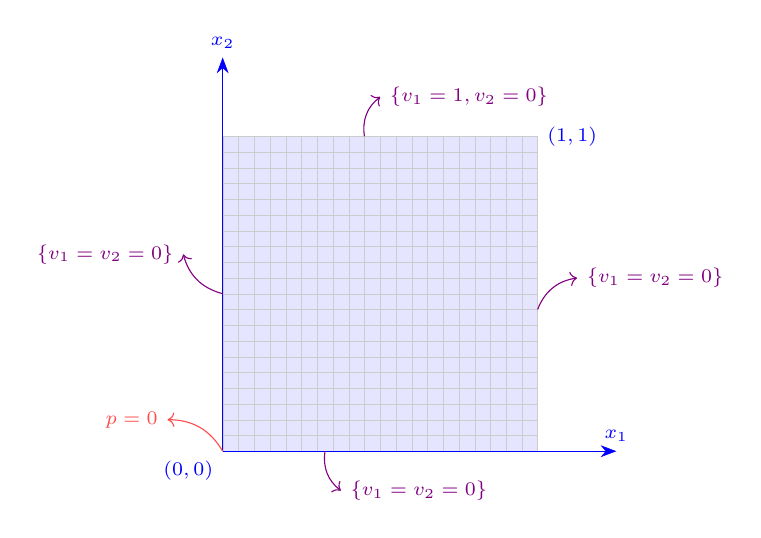
\begin{tikzpicture} [{place/.style={rectangle,draw=blue!50,fill=blue!20,ultra thin,inner sep=0.8mm}},{place2/.style={circle,draw=black!50,ultra thin,inner sep=0.8mm}},{linest/.style={color=gray,ultra thin}}]
	%%coordinates of corners of Beam
	\coordinate (A) at (0,0);
	\coordinate (B) at (4.0,0);
	\coordinate (D) at (4.0,4.0);
	\coordinate (E) at (0.0,4.0);
	
	%% fluid
	\draw [gray!30,fill=blue!10](A) rectangle (D)node [right,color = blue,font=\scriptsize] {$(1,1)$};
	%%mesh
	\draw [line width=0.1pt,gray!40,step=2mm](0,0) grid (D);

	%%axes
	\draw [-{Stealth[length=2mm]},help lines,blue] ($(0,0)$)node [below left,color = blue,font=\scriptsize] {$(0,0)$} -> ($(B)+(1,0)$) node [above,color = blue,font=\scriptsize] {$x_1$};
	\draw [-{Stealth[length=2mm]}, help lines,blue] ($(0,0)$) -> ($(D)+(-4,1)$) node [above,color = blue,font=\scriptsize] {$x_2$};
	

	%%BC
	%% velocity
	\draw [->,violet] (4,1.8) to [bend left] (4.5,2.2)node [right,color = violet,font=\scriptsize] {\{$v_1=v_2=0\}$};
	
	\draw [->,violet] (1.8,4) to [bend left] (2.0,4.5)node [right,color = violet,font=\scriptsize] {\{$v_1=1, v_2=0\}$};
	
	\draw [->,violet] (0,2.0) to [bend left] (-0.5,2.5)node [left,color = violet,font=\scriptsize] {\{$v_1=v_2=0\}$};
	
	\draw [->,violet] (1.3,0) to [bend right] (1.5,-0.5)node [right,color = violet,font=\scriptsize] {\{$v_1=v_2=0\}$};
	%% pressure
	\draw [->,red!70] (0.0,0.0) to [bend right] (-0.7,0.4)node [left,color = red!70,font=\scriptsize] {$p=0$};
	\end{tikzpicture}
\end{document}
	\caption{Geometry, boundary conditions and computational domain used for the analysis.}
	\label{fig_SB}
\end{figure}
There is a discontinuity in the boundary conditions at the two upper corners of the cavity. Two cases can be envisioned: the two upper corners are either considered as belonging to the top mobile side (leaky cavity), or they are assumed to belong to the fixed vertical walls (non-leaky). The former case is adopted here. It introduces a singularity in the pressure field precisely at those two upper corners. Finally, it should be noticed that Dirichlet boundary conditions are imposed on every boundary in this example. This implies that pressure is known up to a constant at an arbitrary point, the lower left corner of the cavity, the value $p = 0$ is prescribed. Here, we solve the lid-driven cavity for the Stokes problem and the standard Galerkin formulation.\cite{donea2003finite}.
\section{Governing Equation} \label{sec: GE} 
In this section we present the governing equations (continuity and momentum) which are in terms of $(\mathbf{v}, P)$ for isotropic, Newtonian, viscous, incompressible fluids in the presence of body forces:
\begin{equation}\label{eq1}
	\begin{aligned}
		&-\nabla \cdot \mathbf{v} = 0\thinspace,\\
		&\rho \Big( \frac{\partial \mathbf{v}}{\partial t } + \mathbf{v} \cdot \nabla \mathbf{v} \Big) + \nabla P - \mu \nabla \cdot \Big[(\nabla \mathbf{v}) + (\nabla \mathbf{v}^T)  \Big]= \rho \mathbf{f}\thinspace.
	\end{aligned}
\end{equation}
where $\mathbf{v}$ represents the velocity vector, $\rho$ is the density, $\mu$ the fluid viscosity and $\mathbf{f}$ is the body force vector measured per unit mass. $P$ is the hydrostatic pressure. The boundary conditions for the flow problem are
given by
\begin{equation}\label{eq2}
	\begin{aligned}
		\mathbf{v} = \mathbf{\bar{v}} \quad \mathrm{on} \ \Gamma_D\thinspace,\\
		\mathbf{t} \equiv \mathbf{\hat{n}} \cdot \boldsymbol{\sigma} = \mathbf{\hat{t}} \quad \mathrm{on} \ \Gamma_N\thinspace.
	\end{aligned}
\end{equation}
where $\mathbf{\hat{n}}$ is the unit normal to the boundary and $\mathbf{\hat{t}}$ is the traction.  The Cauchy stress tensor $\boldsymbol{\sigma}$ can be define as 
\begin{equation}\label{eq3}
	\begin{aligned}
		\boldsymbol{\sigma} = 2\mu \mathbf{D} - P \mathbf{I}
	\end{aligned}
\end{equation}
where $\mathbf{D} = \frac{1}{2} [(\nabla \mathbf{v}) + (\nabla \mathbf{v}^T)]$ and $\mathbf{I}$ is the unit tensor.
\section{Weak Form} \label{sec: WF}
The starting point for the development of the finite element models of Eq.
(\ref{eq1}) is their weak forms. Here we consider steady flow ($\frac{D v}{d t} =0$ ) two-dimensional
case.  The variation formulation of our model problem can be introduced as find $(\mathbf{v},p) \in W$ such that
\begin{equation}\label{eq4}
	\begin{aligned}
		\mathcal{F}(\mathbf{v},P;\mathbf{u},q) = 0 \quad \forall (\mathbf{u},q) \in \hat{W}\thinspace.
	\end{aligned}
\end{equation}
where $W= V \times P$ is a mixed function space, and 
\begin{equation}\label{eq5}
	\begin{aligned}
		\mathcal{F}(\mathbf{v},p;\mathbf{u},q) =\int_{\Omega} \mathbf{u} \nabla P -\mathbf{u}\mu \nabla \cdot \Big[(\nabla \mathbf{v}) + (\nabla \mathbf{v}^T)  \Big] - q \nabla \cdot \mathbf{v} - \mathbf{u}\rho \mathbf{f}\ \mathrm{d}\Omega \thinspace .
	\end{aligned}
\end{equation}
and
\begin{equation}\label{eq6}
	\begin{aligned}
		\hat{W} &= \{\mathbf{u} \in H^1(\Omega) : \mathbf{u} = 0 \text{ on } \Gamma\}, \\
		W &= \{\mathbf{u} \in H^1(\Omega) : \mathbf{u} = 0 \text{ on } (x=0,x=1,y=0), u_2 = 1 \text{ on } y=1 \}\thinspace.
	\end{aligned}
\end{equation}
where $(\mathbf{u},q)$ is a test functions, which will be equated, in the our FE model to the interpolation function used for $(\mathbf{v},P)$. Applying integration by part, and using the definition of stress, we can rewrite the weak form as following
\begin{equation}\label{eq7}
	\begin{aligned}
		0&=-\int_{\Omega^e} q \nabla \cdot\mathbf{v} \mathrm{d}V\thinspace,\\
		0&=\int_{\Omega^e} \mathbf{u}\nabla P - \mathbf{u}\mu \nabla \cdot \Big[(\nabla \mathbf{v}) + (\nabla \mathbf{v}^T)  \Big]
		- \mathbf{u} \rho \mathbf{f} \mathrm{d}V\\
		&=\int_{\Omega^e}\Big\{\nabla \cdot (\mathbf{u}P) - P\nabla  \mathbf{u} \Big\}\mathrm{d}V
		+\int_{\Omega^e}\Big\{ \mu \nabla \mathbf{u} \cdot\Big[(\nabla \mathbf{v}) + (\nabla \mathbf{v}^T)  \Big] - \nabla \cdot \Big(\mathbf{u}\mu \Big[(\nabla \mathbf{v}) + (\nabla \mathbf{v}^T)  \Big]\Big) \Big\}\mathrm{d}V
		-\int_{\Omega^e}\mathbf{u} \rho \mathbf{f} \mathrm{d}V \\
		&= \int_{\Gamma^e} \mathbf{u}P \mathbf{I} \cdot \mathbf{n} \mathrm{d}S
		-\int_{\Omega^e}P\nabla  \mathbf{u} \mathrm{d}V
		-\int_{\Gamma^e} (2\mathbf{u}\mu \mathbf{D}) \cdot \mathbf{n} \mathrm{d}S
		+\int_{\Omega^e}\mu \nabla\mathbf{u}\cdot\Big[(\nabla \mathbf{v}) + (\nabla \mathbf{v}^T)  \Big] \mathrm{d}V
		-\int_{\Omega^e}\mathbf{u} \rho \mathbf{f} \mathrm{d}V\\
		&=-\int_{\Gamma^e} \mathbf{u} \mathbf{\hat{t}}\mathrm{d}S
		-\int_{\Omega^e}P\nabla \mathbf{u} \mathrm{d}V
		+\int_{\Omega^e}\mu \nabla \mathbf{u} \Big[(\nabla \mathbf{v}) + (\nabla \mathbf{v}^T)  \Big] \mathrm{d}V
		-\int_{\Omega^e}\mathbf{u} \rho \mathbf{f} \mathrm{d}V\thinspace.
	\end{aligned}
\end{equation}
\section{Finite Element Model} \label{sec: FEM}
Since we are developing the Ritz-Galerkin finite element models, the choice
of the weight functions is restricted to the spaces of approximation functions
used for the pressure and velocity fields. Suppose that the dependent variables
$(v_i, P )$ are approximated by expansions of the form
\begin{equation}\label{eq8}
	\begin{aligned}
		&v_i(\mathrm{x}, t)= \sum_{m=1}^{M} \psi_m(\mathrm{x}) \mathbf{v}_i^m(t) = \boldsymbol{\Psi}^T\mathbf{v}_i \thinspace,\\
		&p(\mathrm{x}, t)= \sum_{n=1}^{N} \phi_n(\mathrm{x}) P^n(t) = \boldsymbol{\Phi}^T\mathbf{P} \thinspace.
	\end{aligned}
\end{equation}
where $\boldsymbol{\Psi}$ and $\boldsymbol{\Phi}$ are (column) vectors of interpolation (or shape) functions, $\mathbf{v}_i = \{v_1,v_2\}^T$ and
$\mathbf{P}$ are vectors of nodal values of velocity components and pressure, respectively, and the superscript $(\cdot)^T$ denotes a transpose of the enclosed vector or matrix. Substitution of these equation into Eq. (\ref{eq4}) results in the following finite element equations.

Continuity:
\begin{equation}\label{eq9}
	\begin{aligned}
		-\Big[\int \boldsymbol{\Phi} \frac{\partial \boldsymbol{\Psi}}{\partial x_i} \mathrm{d}V \Big] \mathbf{v}_i = 0\thinspace.
	\end{aligned}
\end{equation}

Momentum:
\begin{equation}\label{eq10}
	\begin{aligned}
		\Big[\int_{\Omega^e} \mu  \frac{\partial \boldsymbol{\Psi}}{\partial x_j}  \frac{\partial \boldsymbol{\Psi}^T}{\partial x_j}\mathrm{d}V \Big] \mathbf{v}_i
		+ \Big[\int_{\Omega^e} \mu  \frac{\partial \boldsymbol{\Psi}}{\partial x_j}  \frac{\partial \boldsymbol{\Psi}^T}{\partial x_i}\mathrm{d}V \Big] \mathbf{v}_j
		- \Big[\int_{\Omega^e} \boldsymbol{\Phi}^T \frac{\partial \boldsymbol{\Psi}}{\partial x_i} \mathrm{d}V \Big] \mathbf{P}
		=\int_{\Omega^e} \boldsymbol{\Psi} \rho f_i \mathrm{d}V+\int_{\Gamma^e} \boldsymbol{\Psi} t_i \mathrm{d}S\thinspace.
	\end{aligned}
\end{equation}
The above equations can be written symbolically in matrix form as

\begin{equation}\label{eq11}
	\begin{aligned}
		-\mathbf{Q}^T \mathbf{v} &= \mathbf{0}\thinspace,\\
		\mathbf{K}\mathbf{v} - \mathbf{Q} \mathbf{P}  &= \mathbf{F}\thinspace.
	\end{aligned}
\end{equation}
By combining continuity and  momentum equations into one, Eq. (\ref{eq8}) has the following explicit matrix form:
\begin{equation}\label{eq12}
	\begin{aligned}
		\begin{Bmatrix}
			\mathbf{F_1} \\
			\mathbf{F_2}\\
			0\\
		\end{Bmatrix}
		=&\begin{bmatrix}
			2\mathbf{K}_{11} + \mathbf{K}_{22} & \mathbf{K}_{12} & -\mathbf{Q}_{1} \\
			\mathbf{K}_{21} & \mathbf{K}_{11} +2\mathbf{K}_{22} & -\mathbf{Q}_{2} \\
			-\mathbf{Q}^T_{1} & -\mathbf{Q}^T_{2}  & \mathbf{0} \\
		\end{bmatrix}
		\begin{Bmatrix}
			\mathbf{v_1} \\
			\mathbf{v_2}\\
			\mathbf{P}\\
		\end{Bmatrix}\thinspace.
	\end{aligned}
\end{equation}
The coefficient matrices shown in Eq. (\ref{eq9}) are defined by
\begin{equation}\label{eq13}
	\begin{aligned}
		\mathbf{K}_{ij} = \int_{\Omega^e} \mu \frac{\partial\boldsymbol{\Psi}}{\partial x_i} \frac{\partial\boldsymbol{\Psi}^T}{\partial x_j}\mathrm{d}V\thinspace, \quad \mathbf{Q}_i = \int_{\Omega^e}\frac{\partial\boldsymbol{\Psi}}{\partial x_i} \boldsymbol{\Phi}^T \mathrm{d}V\thinspace, \quad
		\mathbf{F}_i =\int_{\Omega^e} \rho \boldsymbol{\Psi} f_i \mathrm{d}V
		+\int_{\Gamma^e} \boldsymbol{\Psi} t_i \mathrm{d}S \thinspace.
	\end{aligned}
\end{equation}
\section{Choice of Elements} \label{sec: elem}
There are lots of elements available for using in mixed finint elements model, but here for sake of simplicity we choose $Q2Q1$ elements. The quadratic quadrilateral elements shown in Figure \ref{fig_elem} are known to give reliable solutions for velocity and pressure fields.
\begin{figure}[htbp]
	\centering
	\documentclass[preprint,12pt,a4]{standalone}
\usepackage{geometry}   % my added package "geometry"
\geometry{letterpaper,tmargin=1in,bmargin=1in,lmargin=2.5cm,rmargin=2.5cm}
\usepackage{tikz}
\usetikzlibrary{calc,patterns,arrows.meta,shapes.arrows,intersections,positioning}
\usetikzlibrary{decorations.pathmorphing,backgrounds,fit,petri}
\usepackage{standalone}
%
\begin{document}
	\begin{tikzpicture} [{place/.style={rectangle,draw=blue!50,fill=blue!20,ultra thin,inner sep=0.8mm}},{place2/.style={rectangle,draw=black!50,ultra thin,inner sep=0.8mm}},{linest/.style={color=gray,ultra thin}}]
		%axes
		\draw [{Stealth[length=2mm]}-{Stealth[length=2mm]}, help lines,blue] (5.0,0)node[above,font=\scriptsize]{$\xi$} -- (0.0,0.0) -- (0.0,5.0)node[right,font=\scriptsize] {$\eta$};
		%%corner nodes
		\node at (0.0,0.0) [place,fill=violet!60] (1) {};
		\node at (4.0,0.0) [place,fill=violet!60] (2) {};
		\node at (4.0,4.0) [place,fill=violet!60] (3) {};
		\node at (0.0,4.0) [place,fill=violet!60] (4) {};
		%%element border
		\draw [-,black] (1) -- (2) -- (3) -- (4) --(1);
		%%middle nodes
		\node at (2.0,0.0) [place2,fill=gray!60] {};
		\node at (4.0,2.0) [place2,fill=gray!60] {};
		\node at (2.0,4.0) [place2,fill=gray!60] {};
		\node at (0.0,2.0) [place2,fill=gray!60] {};
		\node at (2.0,2.0) [place2,fill=gray!60] {};
		\node at (5.5,3.0) [place2,fill=gray!60] {};
		\node at (5.6,3.0) [right,font=\scriptsize]{$\mathrm{nodes \ with} \ \{v_1, v_2$\}};
		\node at (5.5,2.5) [place,fill=violet!60] (4) {};
		\node at (5.6,2.5) [right,font=\scriptsize]{$\mathrm{nodes \ with} \ \{v_1, v_2, P$\}};
		
	\end{tikzpicture}
\end{document}
	\caption{Quadratic quadrilateral element used for the mixed finite element model.}
	\label{fig_elem}
\end{figure}
\section{Implementation} \label{sec: imp}
In this section, we present the implementation of our solution in the Hiperlife. The program is divided into three separate files, main part which we create our problem by the Hiperlife headers, auxiliary header where we introduce parameters and declare our functions, and at last auxiliary file, where we define some functions which provide required matrices like the Hessian and Jacobian.
\subsubsection{CavityFlow.cpp} \label{sec: m.cpp}
\nolinenumbers
\begin{lstlisting}
/*
* Incompressible stokes flow: Cavity flow problem
*/
// cpp headers
#include <iostream>
#include <fstream>
#include <cmath>

// hiperlife headers
#include "hl_Core.h"
#include "hl_Parser.h"
#include "hl_Tensor.h"
#include "hl_TypeDefs.h"  
#include "hl_DOFsHandler.h"
#include "hl_HiPerProblem.h"
#include "hl_FillStructure.h"
#include "hl_ParamStructure.h"
#include "hl_DistributedMesh.h" 
#include "hl_StructMeshGenerator.h" 
#include "hl_GlobalBasisFunctions.h"
#include "hl_LinearSolver_Direct_MUMPS.h"
#include "hl_NonlinearSolver_NewtonRaphson.h"
#include "hl_LinearSolver_Iterative_AztecOO.h"

// Header to auxiliary functions
#include "AuxCavityFlow.h"

// -------------------------------------------------------------------//
/// -----------------    MAIN FUNCTION     --------------------------///
// -------------------------------------------------------------------//

int main(int argc, char** argv)
{
	using namespace std;
	using namespace hiperlife;
	using namespace hiperlife::Tensor;
	
	// ---------------------------------------------------------------//
	/// *****                 INITIALIZATION                    *****///
	// ---------------------------------------------------------------//
	
	// Initialize MPI
	hiperlife::Init(argc, argv);
	
	// ---------------------------------------------------------------//
	/// *****                   DATA INPUT                      *****///
	// ---------------------------------------------------------------//
	
	// Put parameters in the user structure
	SmartPtr<ParamStructure> paramStr = CreateParamStructure<CavityParams>();
	
	// Data
	paramStr->setRealParameter(CavityParams::rho, 1.0);
	paramStr->setRealParameter(CavityParams::mu, 0.1);
	paramStr->setRealParameter(CavityParams::f1, 0.0);
	paramStr->setRealParameter(CavityParams::f2, 0.0);
	
	double rho = paramStr->getRealParameter(CavityParams::rho);
	double mu = paramStr->getRealParameter(CavityParams::mu);
	double f1 = paramStr->getRealParameter(CavityParams::f1);
	double f2 = paramStr->getRealParameter(CavityParams::f2);
	
	
	// analysis parameter
	ElemType elemType = ElemType::Square;// Triang or Square
	int n = 10;// number of elements in x and y direction 
	// ---------------------------------------------------------------//
	/// *****                   MESH CREATION                   *****///
	// ---------------------------------------------------------------//
	
	// Create a structural mesh       
	SmartPtr<StructMeshGenerator> StrMesh = Create<StructMeshGenerator>();
	StrMesh->setNDim(3);
	StrMesh->setBasisFuncType(BasisFuncType::Lagrangian);
	StrMesh->setBasisFuncOrder(1);
	StrMesh->setElemType(elemType);
	StrMesh->genSquare(n,1.0);
	
	//-------------------Distributed Mesh------------------------------//
	// For Pressure
	SmartPtr<DistributedMesh> disMeshPress = Create<DistributedMesh>();
	
	disMeshPress->setMesh(StrMesh);
	disMeshPress->setBalanceMesh(true);
	disMeshPress->setElementLocatorEngine(ElementLocatorEngine::BoundingVolumeHierarchy);
	disMeshPress->Update();
	
	// For Velocity
	SmartPtr<DistributedMesh> disMeshVeloc = Create<DistributedMesh>();
	
	disMeshVeloc->setMeshRelation(MeshRelation::pRefin, disMeshPress);
	disMeshVeloc->setPRefinement(1);
	disMeshVeloc->setBalanceMesh(true);
	disMeshVeloc->setElementLocatorEngine(ElementLocatorEngine::BoundingVolumeHierarchy);
	disMeshVeloc->Update();
	
	cout << "--check meshv/p files to see the meshes--" << endl;
	disMeshVeloc->printFileLegacyVtk("meshv");
	disMeshPress->printFileLegacyVtk("meshp");
	
	// ---------------------------------------------------------------//
	/// *****               DOFsHANDLER CREATION                *****///
	// ---------------------------------------------------------------//
	
	// DOFHandler
	// For Velocity
	SmartPtr<DOFsHandler> dhandV = Create<DOFsHandler>(disMeshVeloc);
	dhandV ->setNameTag("dhandV");
	dhandV ->setNumDOFs(2);
	dhandV->setDOFs({"vx","vy"});
	dhandV->Update();
	
	// For Pressure
	SmartPtr<DOFsHandler> dhandP = Create<DOFsHandler>(disMeshPress);
	dhandP->setNameTag("dhandP");
	dhandP ->setNumDOFs(1);
	dhandP->setDOFs({"p"});
	dhandP->Update(); 
	cout << "--DOFsHandler for Velocity and Pressure successfully created--" << endl;
	
	
	// ------------------ Boundary conditions------------------------ //
	//---------------------------------------------------------------//
	// Set boundary conditions for the velocity
	//velocities are zero everywhere except at Ymax vx=1
	dhandV->setBoundaryCondition(0, MAxis::Xmin, 0.0);
	dhandV->setBoundaryCondition(1, MAxis::Xmin, 0.0);
	
	dhandV->setBoundaryCondition(0, MAxis::Xmax, 0.0);
	dhandV->setBoundaryCondition(1, MAxis::Xmax, 0.0);
	
	dhandV->setBoundaryCondition(0, MAxis::Ymin, 0.0);
	dhandV->setBoundaryCondition(1, MAxis::Ymin, 0.0);
	
	dhandV->setBoundaryCondition(0, MAxis::Ymax, 1.0);
	dhandV->setBoundaryCondition(1, MAxis::Ymax, 0.0);
	
	// Set boundary conditions for the pressure
	// Set initial value for the pressure at (0,0) p=0  
	dhandP->setBoundaryCondition(0,0,IndexType::Local,0.0);
	
	// Update
	dhandV->UpdateGhosts();
	dhandP->UpdateGhosts();
	
	// ---------------------------------------------------------------//
	/// *****               HIPERPROBLEM CREATION               *****///
	// ---------------------------------------------------------------//
	
	SmartPtr<HiPerProblem> hiperProbl = Create<HiPerProblem>();
	hiperProbl->setParameterStructure(paramStr);
	hiperProbl->setDOFsHandlers({dhandV, dhandP});
	hiperProbl->setIntegration("IntegCavity", {"dhandV", "dhandP"});
	
	if (elemType==ElemType::Square)
	hiperProbl->setCubatureGauss("IntegCavity", 4);
	else if (elemType==ElemType::Triang)
	hiperProbl->setCubatureGauss("IntegCavity", 3);
	
	hiperProbl->setElementFillings("IntegCavity", LS);
	hiperProbl->Update();
	// ---------------------------------------------------------------//
	/// *****                  SOLVER CREATION                  *****///
	// ---------------------------------------------------------------//
	// Create linear solver direct
	SmartPtr<MUMPSDirectLinearSolver> dirsolver = Create<MUMPSDirectLinearSolver>();
	dirsolver->setHiPerProblem(hiperProbl);
	dirsolver->setVerbosity(MUMPSDirectLinearSolver::Verbosity::Extreme);
	dirsolver->setDefaultParameters();
	dirsolver->Update();
		
	// Solve
	dirsolver->solve();
	hiperProbl->UpdateGhosts();
		
	// Update Solution
	dirsolver->UpdateSolution();
	
	// ---------------------------------------------------------------//
	/// *****                Post Processing                 *****///
	// ---------------------------------------------------------------//
	
	// Print solution
	dhandP->printFileLegacyVtk("CavityP");
	dhandV->printFileLegacyVtk("CavityV");
	
	// mpi finilizing
	hiperlife::Finalize();
	return 0;
}
\end{lstlisting}
\subsubsection{AuxCavityFlow.h} \label{sec: a.h}
\begin{lstlisting}
#ifndef AUXCavity_H
#define AUXCavity_H

// C headers
#include <iostream>

// hiperlife headers
#include "hl_Core.h"
#include "hl_Parser.h"
#include "hl_TypeDefs.h"  
#include "hl_DOFsHandler.h"
#include "hl_HiPerProblem.h"
#include "hl_FillStructure.h"
#include "hl_ParamStructure.h"
#include "hl_DistributedMesh.h" 
#include "hl_StructMeshGenerator.h" 
#include "hl_GlobalBasisFunctions.h"
#include "hl_NonlinearSolver_NewtonRaphson.h"
#include "hl_LinearSolver_Iterative_AztecOO.h"

struct CavityParams
{
	enum RealParameters
	{
		rho,
		mu,
		f1,
		f2,
	};
	HL_PARAMETER_LIST DefaultValues
	{
		{"rho,", 1.0},
		{"mu,", 0.1},
		{"f1,", 0.0},
		{"f2,", 0.0},
	};
};

void LS(hiperlife::FillStructure& fillStr);

#endif

\end{lstlisting}
\subsubsection{AuxCavityFlow.cpp} \label{sec: a.cpp}
\begin{lstlisting}
// Header to cpp
#include <fstream>
#include <iostream>
#include <string>

// Header to auxiliary functions
#include "AuxCavityFlow.h"

// Hiperlife headers
#include "hl_Core.h"
#include "hl_ParamStructure.h"
#include "hl_Parser.h"
#include "hl_TypeDefs.h"
#include "hl_GlobalBasisFunctions.h"
#include "hl_StructMeshGenerator.h"
#include "hl_DistributedMesh.h"
#include "hl_FillStructure.h"
#include "hl_DOFsHandler.h"
#include "hl_HiPerProblem.h"
#include "hl_LinearSolver_Iterative_AztecOO.h"
#include "hl_NonlinearSolver_NewtonRaphson.h"

using namespace std;
using namespace hiperlife;
using namespace hiperlife::Tensor;


// Cavity flow

void LS(hiperlife::FillStructure& fillStr)
{
	using namespace std;
	using namespace hiperlife;
	using hiperlife::Tensor::tensor;
	
	double rho  = fillStr.getRealParameter(CavityParams::rho);
	double mu = fillStr.getRealParameter(CavityParams::mu);
	double f1 = fillStr.getRealParameter(CavityParams::f1);
	double f2 = fillStr.getRealParameter(CavityParams::f2);
	ttl::tensor<double,1>  F{f1,f2};
	
	
	//----------------------------------------------------------------//
	// ------------------------- INPUT DATA --------------------------//
	//----------------------------------------------------------------//
	
	//--------------------------Velocity-related----------------------//
	// Dimensions
	SubFillStructure& subFill = fillStr["dhandV"];
	int pDim = subFill.pDim;
	int eNN  = subFill.eNN;
	int numDOFs = subFill.numDOFs;
	
	// Shape functions and derivatives at Gauss points
	double jac{};
	ttl::wrapper<double,2> nborCoords(subFill.nborCoords.data(), eNN, pDim);
	ttl::wrapper<double,2> nborDOFs(subFill.nborDOFs.data(), eNN, numDOFs);
	ttl::tensor<double,1,false>  bf(subFill.nborBFs(), eNN);
	ttl::tensor<double,2> Dbf_g(eNN,pDim);
	GlobalBasisFunctions::gradients(Dbf_g, jac, subFill);
	
	//--------------------------Pressure-related----------------------//
	// Dimensions
	SubFillStructure& subFill_p = fillStr["dhandP"];
	int nDim_p = subFill_p.nDim;
	int eNN_p  = subFill_p.eNN;
	int numDOFs_p = subFill_p.numDOFs;
	
	// Shape functions and derivatives at Gauss points
	ttl::wrapper<double,2> nborCoords_p(subFill_p.nborCoords.data(),eNN_p,nDim_p);
	ttl::wrapper<double,1> nborDOFs_p(subFill_p.nborDOFs.data(),eNN_p);
	ttl::tensor<double,1,false>  bf_p(subFill_p.nborBFs(),eNN_p);
	
	//------------------------------------------------------------------------------//
	// ----------------------------- OUTPUT DATA -----------------------------------//
	//------------------------------------------------------------------------------//
	ttl::wrapper<double,2> Bk0(fillStr.Bk(0).data(),eNN,numDOFs);
	ttl::wrapper<double,1> Bk1(fillStr.Bk(1).data(),eNN_p);
	
	ttl::wrapper<double,4> Ak00(fillStr.Ak(0,0).data(),eNN,numDOFs,eNN,numDOFs);
	ttl::wrapper<double,3> Ak01(fillStr.Ak(0,1).data(),eNN,numDOFs,eNN_p);
	ttl::wrapper<double,3> Ak10(fillStr.Ak(1,0).data(),eNN_p,eNN,numDOFs);
	ttl::wrapper<double,2> Ak11(fillStr.Ak(1,1).data(),eNN_p,eNN_p);
	
	//---------------------------- EQUATIONS -----------------------------------//
	//--------------------------------------------------------------------------//
	for (int i=0;i < eNN;i++)
	{
		for (int j=0;j < eNN;j++)
		{
			Ak00(i,0,j,0)+=jac*mu*(2.0*Dbf_g(i,0)*Dbf_g(j,0)+Dbf_g(i,1)*Dbf_g(j,1));
			Ak00(i,0,j,1)+=jac*mu*Dbf_g(i,1)*Dbf_g(j,0);
			Ak00(i,1,j,0)+=jac*mu*Dbf_g(i,0)*Dbf_g(j,1);
			Ak00(i,1,j,1)+=jac*mu*(2.0*Dbf_g(i,1)*Dbf_g(j,1)+Dbf_g(i,0)*Dbf_g(j,0));
		}
		for (int j=0;j < eNN_p;j++)
		{
			Ak01(i,0,j)-=jac*Dbf_g(i,0)*bf_p(j);
			Ak01(i,1,j)-=jac*Dbf_g(i,1)*bf_p(j);
			
			Ak10(j,i,0)-=jac*bf_p(j)*Dbf_g(i,0);
			Ak10(j,i,1)-=jac*bf_p(j)*Dbf_g(i,1);
		} 
	}
	
}

\end{lstlisting}
\section{Results} \label{sec: rst}
In this section, we present the results of our solution. Figure \ref{fig_Rs1} shows the velocities distribution in our domain.

\begin{figure}[htbp]
	\centering
	\subfloat[\centering velocity in x-direction]{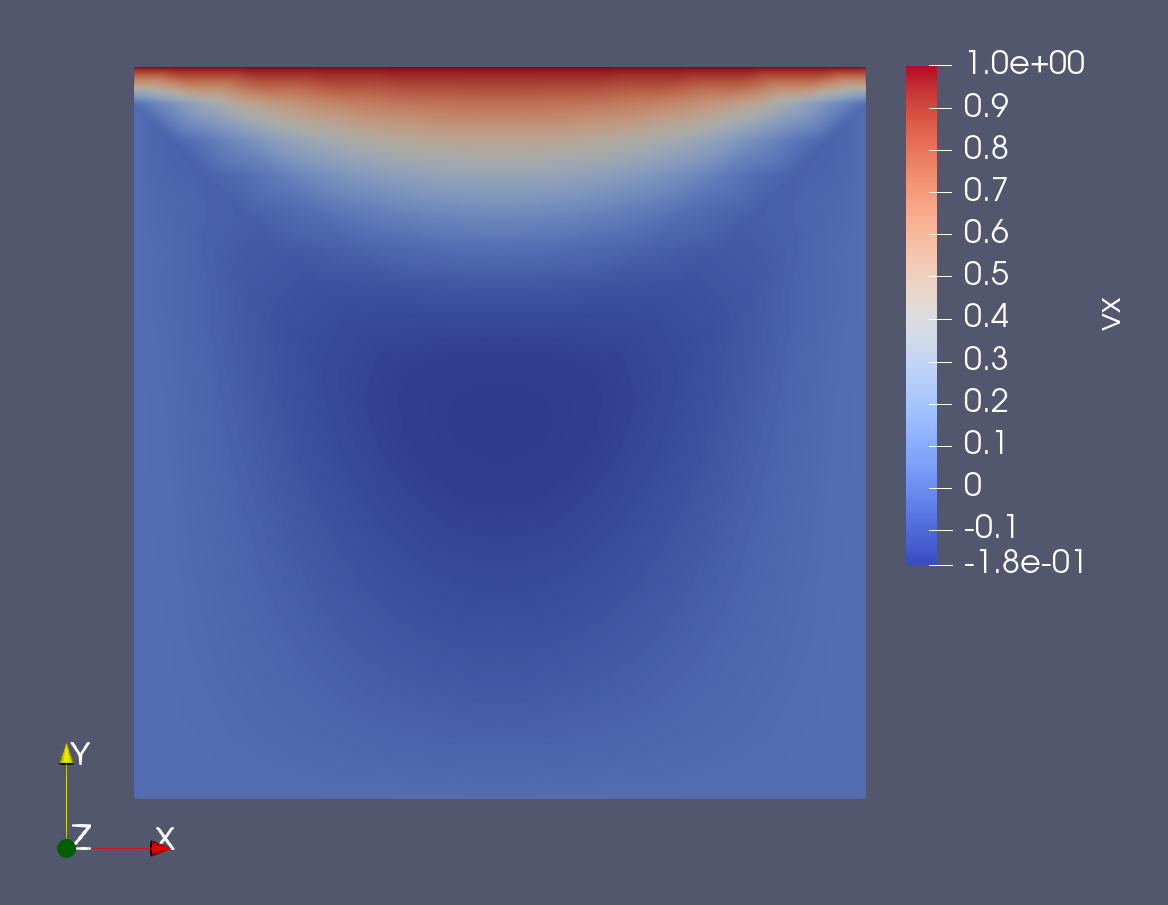
\includegraphics[width=200pt]{Figures/vx.png}}%
	\qquad
	\subfloat[\centering velocity in y-direction]{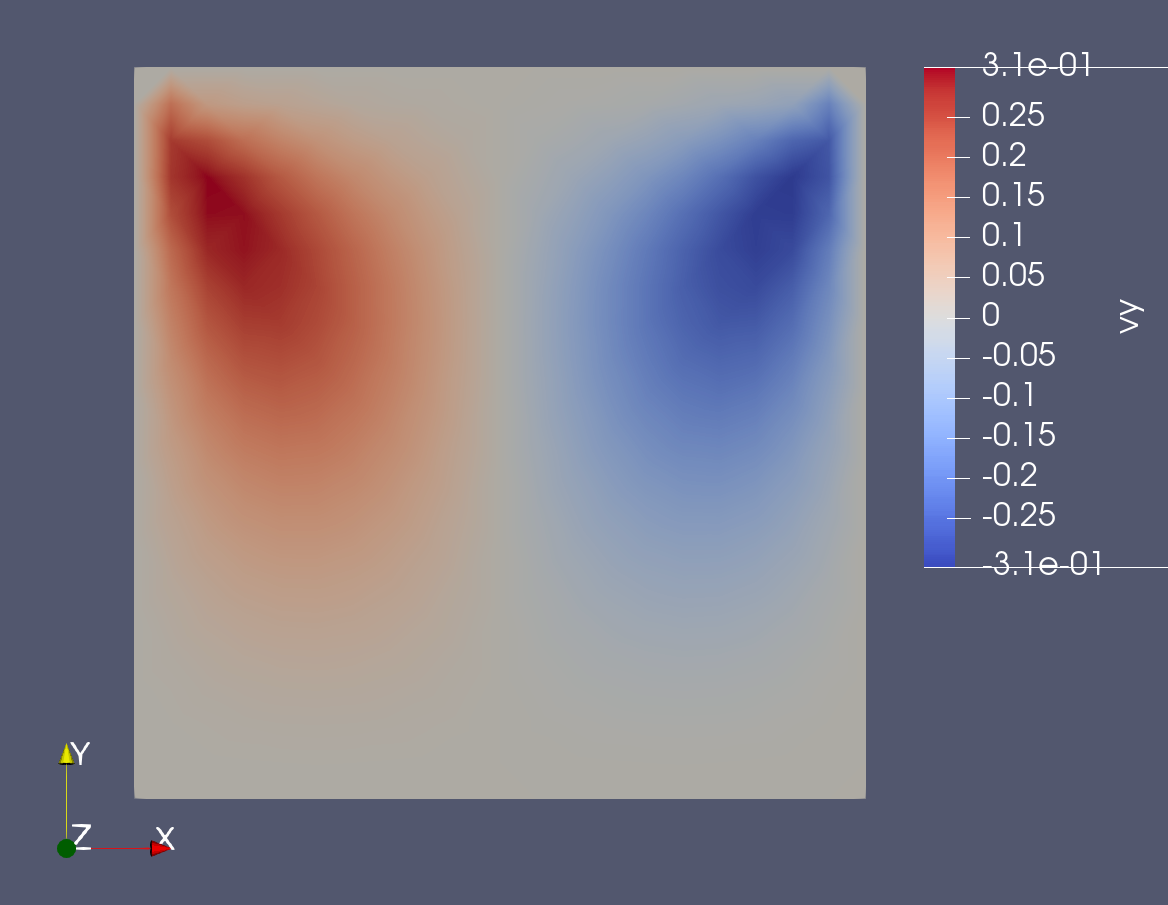
\includegraphics[width=200pt]{Figures/vy.png} }%
	\caption{velocity of flow in cavity}%
	\label{fig_Rs1}%
\end{figure}
Pressure contour is presented in Figure \ref{fig_Rs2}.
\begin{figure}[htbp]
	\centering
	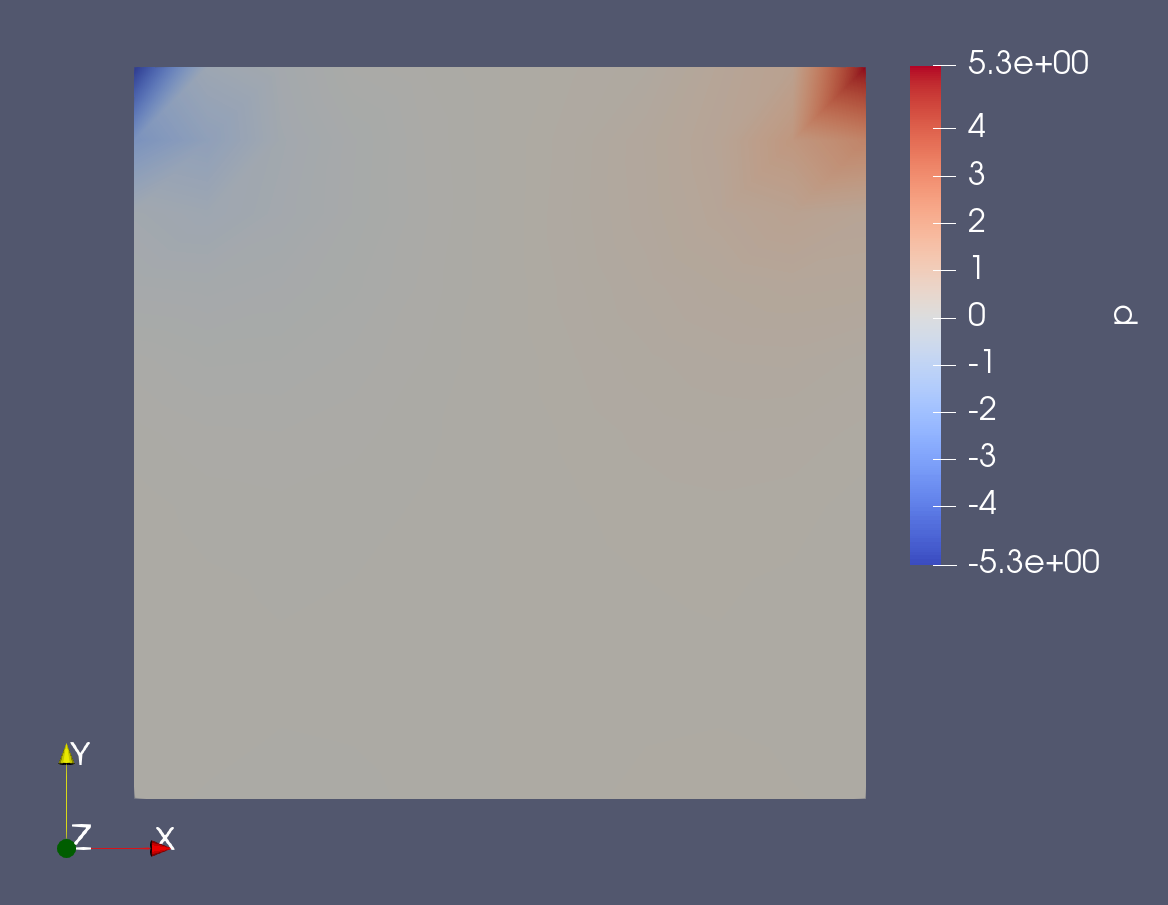
\includegraphics[width=250pt]{Figures/p.png}
	\caption{Pressure distribution in the domain.}
	\label{fig_Rs2}
\end{figure}
\bibliographystyle{unsrt}
\bibliography{ref}
\end{document}
